\begin{surferPage}[Sextic (30 Cusps)]{The Barth Sextic with 30 Cusps}
    After Wolf Barth had constructed the sextic with the maximum possible
    number of singularities, $65$ (see another surface in this gallery) and
    two of his Ph.D.\ students had also constructed new world record surfaces
    for higher degrees, he started to consider the question on the maximum
    number of cusps on surfaces of a given degree.

   Barth's construction of the sextic with $65$ singularities of type
    $A_1^{+-}$ (double cones) can be adapted to cusps, this yields $30$ of
    them: 
    \[P_6 - \alpha \cdot K^3=0,\]
  where $P_6$ are the same symmetry planes of the icosahedron as in the
    other Barth Sextic. As before $K$ is
    again the equation of a unit sphere:
    \vspace*{-0.4em}
    \begin{center}
      \begin{tabular}{c@{\ }c@{\ }c@{\ }c}
        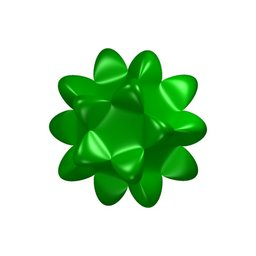
\includegraphics[height=1.2cm]{./../../common/images/barthsextic_30A2}
        &
        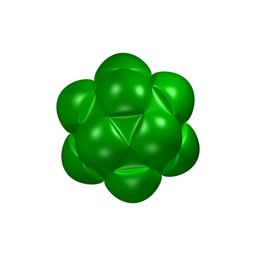
\includegraphics[height=1.2cm]{./../../common/images/barthsextic_30A2_3}
        &
        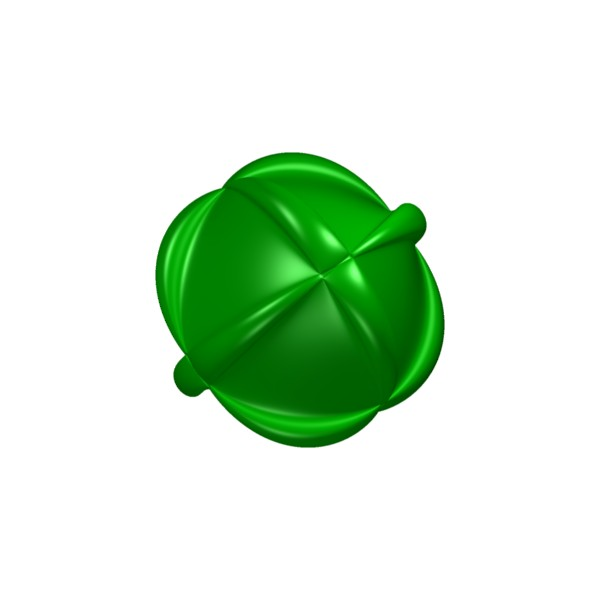
\includegraphics[height=1.2cm]{./../../common/images/barthsextic_30A2_5}
        &
        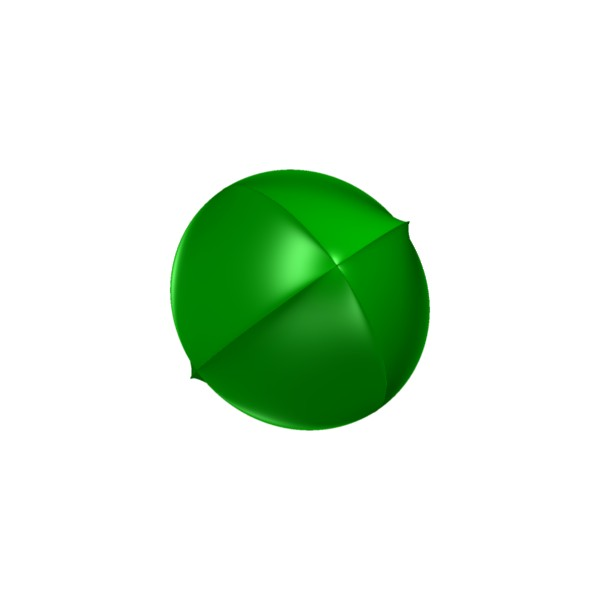
\includegraphics[height=1.2cm]{./../../common/images/barthsextic_30A2_6}
      \end{tabular}
    \end{center}    
    \vspace*{-0.3em}
     This is the current world record for the maximum number of real cusps on
    sextics, for complex cusps, it is $36$.
\end{surferPage}
